\documentclass{report}

% Language setting
% Replace `english' with e.g. `spanish' to change the document language
\usepackage[english]{babel}

% Set page size and margins
% Replace `letterpaper' with `a4paper' for UK/EU standard size
\usepackage[letterpaper,top=2cm,bottom=2cm,left=3cm,right=3cm,marginparwidth=1.75cm]{geometry}

% Useful packages
\usepackage{amsmath}
\usepackage{graphicx}
\usepackage[colorlinks=true, allcolors=blue]{hyperref}

\newtheorem{definition}{Definition}[section]

\title{Protein Structures}
\author{Vinay Kakkar}

\begin{document}
\maketitle

\tableofcontents

\begin{abstract}
Abstract here!
What the report is about
Short part to explain why we need this report
\end{abstract}

\section{Introduction}
Amino acids are molecules that combine to form proteins. All of the 20 amino acids see table~\ref{Amino acids} have in common a central carbon atom which are attached a hydrogen atom, an amino group and a carboxyl group. What distinguishes one amino acid from
another is the side chain attached to the central carbon atom through its fourth valence~\cite{branden_introduction_1998}.

\begin{table}[h!]
    \begin{center}
    \label{tab:Amino acids}
        \begin{tabular}{l|c|r}
        Amino acid & Three-letter code & One-letter code\\
        \hline
        \\
        Glycine & Gly & G\\
        Alanine & Ala & A\\
        Valine & Val & V\\
        Leucine & Leu & L\\
        Isoleucine & Ile & I\\
        Proline & Pro & P\\
        Phenylalanine & Phe & F\\
        Methionine & Met & M\\
        Tryptophan & Trp & W\\
        Cysteine & Cys & C\\
        \\
        \hline
        \\
        Asparagine & Asn & N\\
        Glutamine & Gln & Q\\
        Serine & Ser & S\\
        Threonine & Thr & T\\
        Tyrosine & Tyr & Y\\
        \\
        \hline
        \\
        Aspartic acid & Asp & D\\
        Glutamic acid & Glu & E\\
        \\
        \hline
        \\
        Histidine & His & H\\
        Lysine & Lys & K\\
        Arginine & Arg & R\\
        \end{tabular}
        \caption{\label{Amino acids}The 20 amino acids. The amino acid name, the three-letter code, and the one-letter code are given. The Amino acids are split up into Nonpolar, Polar, Acidic and Basic respectfully}
    \end{center}
\end{table}

Proteins are responsible of catalysing almost all the chemical reactions in the cell. Proteins can function as enzymes catalysing a wide variety of reactions vital for life thus being important for the structure of living systems such as those proteins involved in the cytoskeleton. The size of protein can vary from small to quite large macromolecules~\cite{zvelebil_understanding_2008}.

\begin{definition}[Catalysing]
    Catalysing is to make a chemical reaction happen or happen more quickly by acting as a catalyst.
\end{definition}

\begin{definition}[Cytoskeleton]
    A dynamic network of interlinking protein filaments present in the cytoplasm of all cells~\cite{zvelebil_understanding_2008}. 
\end{definition}

Given that protiens are a built up off of amino acids, we can analyse a DNA sequence of a gene to retrieve the amino acid sequence of the protein product. Using this and Bioinformatics we can help deduce the likely properties of unknown proteins, whilst including their functions and structures. Knowing the relationship between a proteins structure and its function provides a greater understanding of how the protein works and thus enables experiments to explore how modifying the structure will affect the function. Interacting with proteins, structure-function studies are vital to the design of new drugs, the use of bioinformatics exelerates this process aswell as providing computer modelling of these interactions~\cite{zvelebil_understanding_2008}.

\section{Protein Structure}

\subsection{Primary and Secondary Structure}

\subsubsection{Protein structure can be considered on several different levels}

A protein folds into a three-dimensional structure, which is determined by its protein sequence. The fold of the protein consists of repeating structural units called secondary structures. The fold of the protein is very important for the way the protein will function, and whether it will function correctly. Therefore the study of the ways in which proteins fold and understanding how they fold is an important area of bioinfor- matics, as well as predicting the fold of a protein from its sequence~\cite{zvelebil_understanding_2008}.

Protein structure can be considered on several different levels
The analysis of protein structure by experimental techniques such as X-ray crystal- lography and nuclear magnetic resonance (NMR) has shown that proteins adopt distinct structural elements. The primary structure is the protein sequence, the types and order of the amino acids in the protein chain. the secondary structure is the first level of protein folding, in which parts of the chain fold to form generic structures that are found in all proteins. The tertiary structure is formed by the further folding and packing together of these elements to give the final three-dimensional conformation unique to the protein. Many functional proteins are formed of more than one protein chain, in which case the individual chains are called protein subunits~\cite{zvelebil_understanding_2008}. 

The subunit composition and arrangement in such multisubunit proteins is called the quaternary conformation. The structure adopted by a protein chain, and thus its function, is determined entirely by its amino acid sequence, but the rules that govern how a protein chain of a given sequence folds up are not yet understood and it is impossible to predict the folded structure of a protein de novo from its amino acid sequence alone. Helping to solve this problem is one of the challenges facing bioinformatics~\cite{zvelebil_understanding_2008}.

De novo: The first occurrence of cancer in the body

\begin{figure}
    \centering
    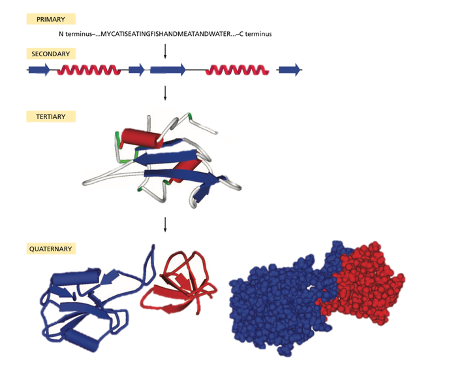
\includegraphics[width=0.5\textwidth]{Protein Structure.png}
    \caption{\label{fig:Simple schematic showing the different levels of protein structure.}From the sequence alone (the primary structure) to secondary structure (which contains local structural elements), to tertiary structure (where the structural elements fold to give a three-dimensional structure), to finally quaternary structure found when several tertiary structures form a multisubunit complex~\cite{zvelebil_understanding_2008}.}
\end{figure}

Amino acids are the building blocks of proteins
Proteins are made up of 20 types of naturally occurring amino acids with a few other amino acids occurring infrequently. of an amino acid can be divided into a common main chain part and a side chain that differs in chemical structure among the different amino acids. The side chain is attached to the main chain carbon atom known as the a-carbon~\cite{zvelebil_understanding_2008}.

The differing chemical and physical properties of amino acids are due to their side chains. The functional properties of proteins are almost entirely due to the side chains of the amino acids. Each type of amino acid has specific chemical physical properties that are conferred on it by the structure and chemical properties of its side chain. They can, however, be classified into overlapping groups that share some common physical and chemical properties, such as size and electrical charge. Some side chains can be charged and not charged they can even be negatively or positively charged~\cite{zvelebil_understanding_2008}.

Amino acids are covalently linked together in the protein chain by peptide bonds. The primary structure of a protein is the sequence of amino acids in the linear protein chain, which consists of covalently linked amino acids. This linear chain is often called a polypeptide chain~\cite{zvelebil_understanding_2008}.

\begin{figure}
    \centering
    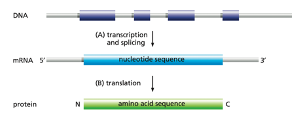
\includegraphics[width=0.5\textwidth]{Transcription and translation.png}
    \caption{\label{fig:Transcription and translation}The relation of DNA coding-strand sequence to mRNA sequence to protein sequence. The exons (purple boxes) of the DNA are transcribed into mRNA which, using other molecules directs the protein sequence~\cite{zvelebil_understanding_2008}.}
\end{figure}

Secondary structure of proteins is made up of a-helices and b-strands
It should be noted that the structures found in globular proteins are not perfectly regular, so it is frequently difficult to define the precise ends of the helices, and in some cases the hydrogen-bonding patterns are intermediate between these idealized forms. Therefore, prediction of these structures using bioinformatics programs is made more difficult~\cite{zvelebil_understanding_2008}.

Several different types of b-sheet are found in protein structures. Turns, hairpins, and loops connect helices and strands. Any chain between two regular structures is referred to as a loop. In many cases a loop will contain a turn (or even several). In general there are no classifications for loops, but there is an important exception. In antibody recognition, immunoglobulins employ loops at the edge of a b-sheet to recognize the antigen. There are vast numbers of different immunoglobulin structures, all with the same overall chain fold, but it is the difference at these loops that results in different affinities. With many structures known, it has been observed that the loops take up one of a limited number of structures (called canonical forms), so that in this particular case the loops have been classified. This type of classification is important when trying to predict both the structure and function of the protein~\cite{zvelebil_understanding_2008}.

\subsection{Proteins Fold to Form Compact Structures}

Protein chains themselves rarely have any biological function. Only when the chain has folded up into a three-dimensional structure (however small) does the protein have functional activity. Some proteins are enzymes that bind other molecules (ligands) and catalyze their biochemical reactions, others act by binding other proteins and influencing their activity, and yet others bind to DNA and regulate gene expression. Some proteins have a purely structural function, making up the fabric of the cell. Large numbers of proteins are released, or secreted, from cells and act as chemical messengers, influencing the behavior of other cells by acting on yet another large functional class of proteins, known as receptors, on cell surfaces~\cite{zvelebil_understanding_2008}.

The tertiary structure of a protein is defined by the path of the polypeptide chain
In the tertiary structure of a protein, various combinations of secondary structure pack together to form a compactly folded mass. In a multidomain protein it is thought that each domain folds independently of the others. Bioinformatics questions are often concerned with comparing the sequences and structures of different domains rather than whole proteins. A domain can be anything from 50 to around 350 amino acids in length. The core of each domain is mainly composed of tightly packed a-helices, b-sheets, or a mixture of both. The three- dimensional structure of a protein is known as its conformation. More specifically, the spatial path of any given folded polypeptide chain is known as its fold~\cite{zvelebil_understanding_2008}.

As proteins exist in an aqueous environment, folding tends to result in hydrophobic regions of the protein ending up in the interior, while more hydrophilic regions are on the outside. A variety of noncovalent interactions stabilize the fold, dominated by hydrogen bonding and the clustering of hydrophobic groups. Secondary structures pack together in a variety of ways, such as the formation of b-sheets from either parallel or antiparallel b-strands. The atoms pack together very efficiently in most natural proteins~\cite{zvelebil_understanding_2008}.

There appears to be a limited number of ways in which secondary structures fold into domains. There are several instances where proteins that seem to be completely unrelated in terms of sequence are found to have the same fold and some researchers estimate that there may be only a few thousand different folds in nature. Currently, there are more than 35,000 known protein structures, and these are classified into approximately 2000 fold families. The fact that so many proteins fold into a similar structure even if their sequences are not very similar means that we can use bioinformatics tools to model structures of various proteins on similar folds~\cite{zvelebil_understanding_2008}.

The stable folded state of a protein represents a state of low energy. A protein chain starts to fold as soon as it has been synthesized and thermodynamic considerations mean that the final fold it adopts is a state of low free energy. Folded proteins are generally stable in the conditions in which they have to operate, but in a wider sense, proteins are unstable thermodynamically. Most proteins start to unfold above about 60C, as the noncovalent bonds that hold them together are broken by thermal energy; unfolded proteins are said to be denatured. As it becomes denatured, a protein loses its function. Only specialized microorganisms are capable of living at temperatures this high~\cite{zvelebil_understanding_2008}.

Many proteins are formed of multiple subunits. Individual folded polypeptides can interact with each other to form protein complexes or quaternary structures~\cite{zvelebil_understanding_2008}.

\section{Large Scale Experssion}

Gene expression begins when genes are transcribed into messenger RNAs (mRNAs), which are then translated to produce proteins. Total gene expression in cultured cells or a tissue sample can be detected in two main ways. One is the detection and quantification of total messenger RNA—the transcriptome—by DNA microarray technology. The other detects the total protein composition of the sample—the proteome—by separating the protein products of the genes by two-dimensional gel electrophoresis or chromatography, followed by identification of their constituent peptides by mass spectrometry. In both these cases a single experiment produces enormous amounts of raw data, and new techniques had to be devised for data collection, storage, and analysis. The transcriptome and proteome, unlike the genome, are changeable in response to conditions, and depend on the state of development, the environment, and the type of tissue~\cite{zvelebil_understanding_2008}.

Monitoring the simultaneous expression of multiple genes provides information that cannot be obtained by monitoring the expression of one or a few genes at a time. By revealing which genes are expressed together, or co-expressed, for example, these techniques can identify genes that may be functionally related, such as the various members of a multiprotein complex or a metabolic or signalling pathway. This information can be used to help assign possible functions to unidentified genes with the same expression patterns. Co-expression can also help indicate which genes are under the control of the same regulatory system~\cite{zvelebil_understanding_2008}.


\subsection{Large Scale Gene Expression}

High-throughput, whole-genome DNA microarrays have become a very useful tool in biological research. However, the interpretation of the large amount of data produced by a microarray experiment or a series of experiments can be time consuming. It is also difficult because different methods can yield alternative conclu- sions. The aim of these experiments is usually to extract some biological or functional meaning from the lists of genes, either by identifying critical genes that might be responsible for a biological effect, or by finding patterns within the genes that point to an underlying biological process and annotating each one of the genes~\cite{zvelebil_understanding_2008}.

\subsubsection{Serial analysis of gene expression}

first, that a short sequence (a tag) contains enough information to uniquely identify a gene (provided that the tag is obtained from a unique position within each gene); second, that the sequence tags from the total cellular RNA (converted into cDNA) can be linked together to form long DNA molecules, called concatemers. This DNA sequence is read and counted. The total number of times a particular tag is observed in the concatemers approximates the expression level of the corresponding gene (see Figure 15.3). The data produced by SAGE include a list of the tags with their corresponding counts, providing a digital output of cellular gene expression that can easily be analyzed further. The SAGE analysis programs SAGEmap and xProfiler are available on the NCBI website and allow the user to specify which organ is to be investigated. Libraries consisting of gene lists organized by the various types of tissues or cell lines are provided for further choice. The expression associated with these gene lists can be divided into two groups and compared with each other. The output from SAGE provides the SAGE tag, the UniGene ID (Identification number), the gene description, and color- and letter-coded differences in expression levels~\cite{zvelebil_understanding_2008}.

\subsubsection{Detect differential gene expression}

Another alternative to microarrays for looking at differential gene expression in some circumstances is purely computational. Digital differential display (DDD) is a method for comparing EST-based expression profiles in different tissues or condi- tions from various libraries or between pools of EST libraries. An EST library contains short sequences cloned from the total cellular mRNA (converted to cDNA) of a particular tissue or particular condition. The theory is that genes expressed at a high level will be represented by more ESTs than those expressed at a lower level. Genes whose expression levels differ significantly from one set of EST libraries to the next are identified using a statistical test~\cite{zvelebil_understanding_2008}.

The NCBI’s UniGene database forms the core of the DDD method. In UniGene, all the human EST sequences in the databases have been put into distinct clusters, where each cluster represents a single gene. The DDD methods then compare the number of sequences from each EST library assigned to a particular UniGene cluster, and identifies those differences between the clusters that are likely to be biologically significant. The user can select EST libraries from a list on the DDD Web page and may combine selected libraries into specific pools. Figure 15.4 shows a DDD analysis of two selected pools. Each of the three columns on the left repre- sents a particular pool, and the rows represent UniGene clusters. On the right is the gene description, which gives the name of the cluster, and the UniGene ID number for that cluster. Clicking on this ID provides a summary report for that cluster~\cite{zvelebil_understanding_2008}.

\subsubsection{Clustered gene expression data}

Clustered data on gene expression patterns obtained from either gene expression microarrays or genome bioinformatics can be used as a predictive tool to identify new transcription factors or other cell-regulatory proteins. Regulatory elements are identified using both gene expression patterns and the clustering of genes according to function, based on functional annotations obtained experimentally or from sequence homology. The clustered genes (or proteins) can be analyzed with respect to protein–protein interaction data to see if the genes can form a function- ally related pathway. For example, Figure 15.10 illustrates how a cluster identified by SOM clustering (node 0, see list in Figure 15.8B) has been subjected to the pSTIING database to obtain an interaction map. We can see that many of the genes submitted (in red) are connected either directly or through another interaction partner. Therefore it is likely these genes are part of a specific functional pathway. Some of the genes form individual clusters. They may be connected via a gene product (protein) that has not been identified as significantly changed, or may not be on the actual chip. The map can be extended to see if other connections can be found (see Figure 15.10B). In such ways a more complete pathway or interaction map can be generated~\cite{zvelebil_understanding_2008}.

A vast collection of data from many gene expression and protein expression exper- iments is now freely available on the Web and can be mined for biological reanalysis or used as reference data for the development of new bioinformatics tools. For example, the L2L tool is a repository of microarray data that users can search with their own up- or downregulated gene list to see if anyone else has got a similar gene expression pattern~\cite{zvelebil_understanding_2008}.

\subsection{Large Scale Protein Expression}

The proteome refers to all the proteins that make up an organism or, on a smaller scale, the total number of proteins found in a particular cell type at a specific point in time and under specific conditions. An organism will have different protein expression in various parts of its body. The protein expression will also differ between the separate stages of an organism’s life cycle and under different environmental conditions. To understand how an organism or a cell functions both under normal and abnormal (such as disease) conditions it is important to know how protein expression is affected~\cite{zvelebil_understanding_2008}.

\subsubsection{Clustering methods to identify protein spots with similar expression patterns}

As with gene expression data, clustering is a useful method of grouping similar gels or spots together and extracting protein expression patterns that can indicate biological differences or similarities between samples. Many of the clustering methods used for microarray data can be applied to 2D gel data. Figure 15.16 shows an unrooted hierarchical clustering tree constructed from 2D gel data from Swiss 3T3 cells that were stimulated with different growth factors at different times. Protein synthesis after the various stimulation regimes, or with no stimulation, was measured and compared using 2D gels and then analysed by hierarchical clustering. In this instance, the gels clearly fall into two groups (see Figure 15.16). One group cluster on the same main branch as the unstimulated sample, suggesting that these treatments had little effect on protein expression. The other branch clusters together those samples that were stimulated for a longer time and those that were stimulated by more than one growth factor and platelet-derived growth factor (PDGF)~\cite{zvelebil_understanding_2008}.

\section{Alpha Fold}

AlphaFold is a major advancement with the aim to predict a protein’s structure from its amino acid sequence alone. In nature, proteins reliably fold into precise 3D conformations that is critical for its function based on nothing more than the sequence of amino acids that it is composed of. 

In fact, mutations in proteins that lead to misfolding are often associated with disease states, for example, Alzheimer’s and Parkinson’s. 

However, we have not been able to understand this folding process nor predict the 3D shape of a protein based on its sequence alone~\cite{felix_brief_nodate}.

The final output of AlphaFold is a file containing the 3D coordinates for every non-hydrogen atom in the protein. It also outputs a graph showing the confidence levels for every amino acid residue, which allows users to assess the reliability of the predicted structure~\cite{felix_brief_nodate}.

The AlphaFold network directly predicts the 3D coordinates of all heavy atoms for a given protein using the primary amino acid sequence and aligned sequences of homologues as inputs (Fig. 1e; see Methods for details of inputs including databases, MSA construction and use of templates)~\cite{jumper_highly_2021}.

Predicting the 3D structure of protein chains from their primary sequence of amino acids is a fundamental open problem in computational molecular biology. Any approach to this problem must deal with the basic fact that protein structures are invariant under translations and rotations. AlphaFold is a step towards to solve this issue~\cite{baldi_principled_nodate}.

\subsection{AlphaFold 2}

Recently, in the CASP14 experiment, AlphaFold2 (AF2) reached an unprecedented performance level in structure prediction of single-chain proteins16. Thanks to an advanced deep learning model that efficiently utilises evolutionary and structural information, this method consistently outperformed all competitors, reaching an average score of 9016. Recently, RoseTTAFold was developed, trying to implement similar principles17. Since then, other end-to-end structure predictors have emerged using different principles such as fast multiple sequence alignment (MSA) processing in DMPFold218 and language model representations19~\cite{bryant_improved_2022}.

\section{Implication for Bioinformatics}

In part, bioinformatics concerns itself with the analysis of protein sequence to predict the secondary structure, the tertiary structure, and the function of the protein, as well as its relationship to other proteins. Different secondary structures tend to have subtle differences in chemical environments, resulting in amino acid preferences. In addition, amino acid preferences are seen at particular locations in proteins due to the functional role they play, for example as catalytic residues or stabilizing the overall protein structure~\cite{zvelebil_understanding_2008}.

Certain amino acids prefer a particular structural unit
Due to the various properties of the amino acid side chains, certain residues or certain types are found more often in one or the other of the structural units~\cite{zvelebil_understanding_2008}.

Evolution has aided sequence analysis
Protein sequence similarity is a powerful tool for characterizing protein function and structure since an enormous amount of information is conserved throughout the evolutionary process. Sequence alignment and database search techniques can identify homologous proteins. Homologous proteins usually have a similar three-dimensional structure with related active sites and binding domains. Therefore homologous proteins will also often have related functions, although this is not always the case. Most amino acids that change during evolution are found in regions that are not structurally or functionally important, such as many of the loops (or variable) regions. f the homologous protein is also functionally related then the amino acids involved in function are often conserved during evolution, which helps in identifying the function of a new protein~\cite{zvelebil_understanding_2008}.

Homologous: Proteins that have a common ancestor

Visualization and computer manipulation of protein structures
There are a number of programs available that read the coordinate file and convert it to a visible three-dimensional representation of the protein. The protein can be rotated, specific regions highlighted, and some measurements can be calculated. Some of these programs are very powerful and can be of great use in analyzing the structural properties and molecular function, as well as allowing for the manual modification of the molecule. Some of the programs are free or low cost, such as Chimera, Yasara, and DeepView. Others are extremely powerful programs that allow the user to carry out computationally intensive modifications to the molecule, but are expensive~\cite{zvelebil_understanding_2008}.


\bibliographystyle{alpha}
\bibliography{bibliography}


\end{document}